\documentclass[12pt]{report}
\usepackage{graphicx}
\title{COMP24412 Lab 3 - The Riddle of Steel Report}
\author{Tejas Chandrasekar}
\begin{document}
\maketitle
\newpage

\section{Lexical Analysis}
Steel is alloy of iron and carbon, and sometimes other elements. Because of
its high tensile strength and low cost, it is a major component used in
buildings, infrastructure, tools, ships, automobiles, machines, appliances, and
weapons.\par
\begin{enumerate}
  \item POS tagging the above sentence:
  \begin{itemize}
    \item NN: Noun, singular or mass
    \begin{itemize}
      \item steel
      \item alloy
      \item iron
      \item carbon
      \item strength
      \item cost
      \item component
      \item infrastructure
    \end{itemize}
    \item NNS: Noun, plural
    \begin{itemize}
      \item elements
      \item buildings
      \item tools
      \item ships
      \item automobiles
      \item machines
      \item appliances
      \item weapons
    \end{itemize}
    \item JJ: Adjectives
    \begin{itemize}
      \item other
      \item high
      \item tensile
      \item low
      \item major
    \end{itemize}
    \item RB: Adverb
    \begin{itemize}
      \item sometimes
    \end{itemize}
    \item CC: Coordinating conjunction
    \begin{itemize}
      \item Because
      \item and
    \end{itemize}
    \item DT: Determiner
    \begin{itemize}
      \item an
      \item a
      \item its
    \end{itemize}
    \item IN: Preposition/subordinating conjunction
    \begin{itemize}
      \item in
      \item of
    \end{itemize}
    \item VBD: Verb, past tense
    \begin{itemize}
      \item Used
    \end{itemize}
    \item VZD: Verb, 3rd person singular present
    \begin{itemize}
      \item is
    \end{itemize}
    \item PP\$: Possessive pronoun
    \begin{itemize}
      \item it
    \end{itemize}
  \end{itemize}
  \item Pronominal co-references: steel, it
\end{enumerate}

\section{C-Structures}
Sentence is 'Steel is an alloy of iron and carbon, and sometimes other
elements.'.
\begin{enumerate}
  \item Constituency structure: see Figure 1.
  \begin{figure}[ht]
    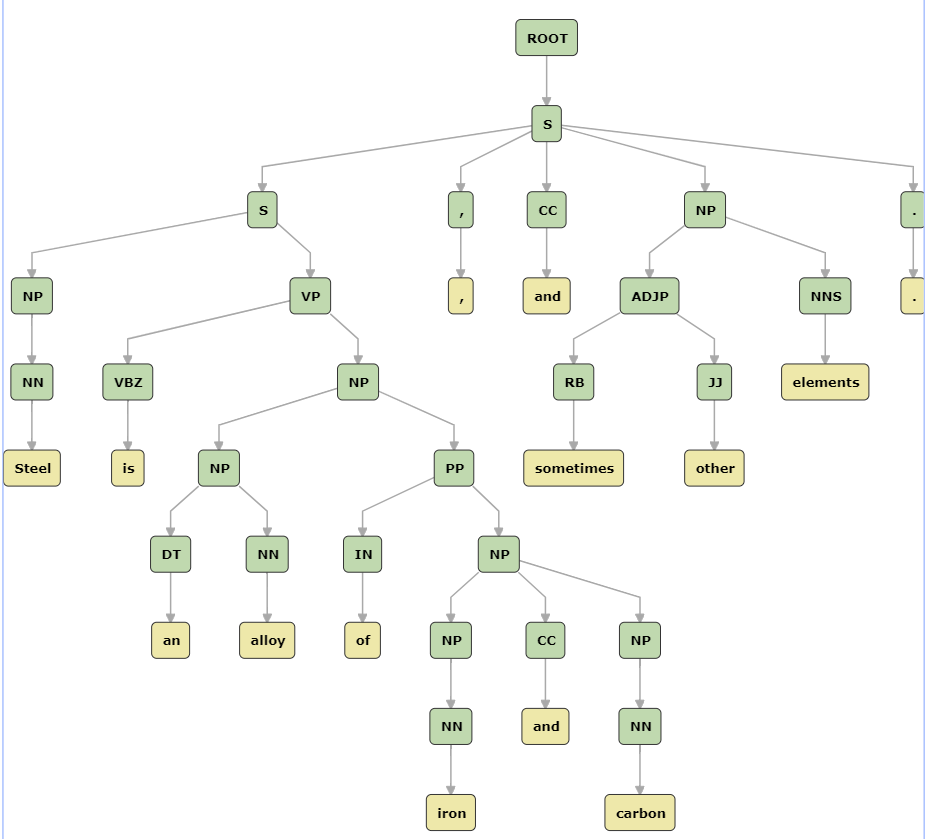
\includegraphics[width=\linewidth]{task2img.PNG}
    \caption{C-strcuture for the sentence}
    \label{Cstruct}
  \end{figure}
  \item Nominal phrasal nodes:
  \begin{itemize}
    \item Steel
    \item an alloy of iron and carbon
    \begin{itemize}
      \item an alloy
      \item iron and carbon
      \begin{itemize}
        \item iron
        \item carbon 
      \end{itemize}
    \end{itemize}
    \item sometimes other elements
  \end{itemize}
  \item Co-ordinations:
  \begin{itemize}
    \item Coordinating conjunction: '...iron AND carbon, AND...'
    \item Gapped coordination: '...sometimes other elements.'
  \end{itemize}
\end{enumerate}

\section{Dependencies - Exploring new territories}
\begin{enumerate}
  \item Constituency parsing divides text into sub-phrases. Using a tree
  structure, the types of phrases belong on branches, the individual words in
  the sentence are leaves, and the designation 'Sentence' is the root.\par

  \noindent Dependency parsing connects words according to their relationships.
  Again using a tree structure, each node in the tree represents a word, with
  the leaf nodes being 'dependent' on the internal nodes, which are most often
  verbs.
  \item Dependency structure: see Figure 2.
  \begin{figure}[h]
    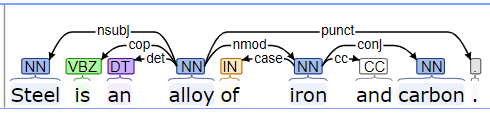
\includegraphics[width=\linewidth]{task3dep.PNG}
    \caption{Dependency structure for sentence: 'Steel is an alloy of iron and
    carbon'}
    \label{DepStruct}
  \end{figure}
\end{enumerate}

\section{Open IE - Semantics}
\begin{enumerate}
  \item Here are the predicate-argument structures for the following sentences:
  \begin{enumerate}
    \item 'Steel is an alloy.': Entity(Steel) $\leftarrow$ Subject --
    relation(is) -- Object $\rightarrow$ (an alloy) Entity(alloy).
    \item 'Steel contains carbon.': Entity(Steel) $\leftarrow$ Subject --
    relation(contains) -- Object $\rightarrow$ (carbon) Entity(carbon).
    \item 'Steel contains iron.': Entity(Steel) $\leftarrow$ Subject --
    relation(contains) -- Object $\rightarrow$ (iron) Entity(iron).
  \end{enumerate}
  \item Prolog translation of triples:\par
    steel(X) :- alloy(X), contains(X, carbon), contains(X, iron).
  \item RDF translation of triples:
  \begin{enumerate}
    \item $\langle Steel \rangle$ $\langle is an \rangle$
    $\langle alloy \rangle$ .
    \item $\langle Steel \rangle$ $\langle contains \rangle$
    $\langle carbon \rangle$ .
    \item $\langle Steel \rangle$ $\langle contains \rangle$
    $\langle iron \rangle$ .
  \end{enumerate}
  \item Axiom formalisation using Description Logics: \par
    Steel$\equiv$ alloy $\sqcap$ hasCarbon $\sqcap$ hasIron
  \item 'Steel is an alloy of iron and carbon.' - as per the next figure, the
  predicate-argument structure is more complex, and the Prolog itself might
  differ like so:\par
    steel(X) :- alloy(X, [carbon, iron]).\par

    Previously, the three separate statements simply translated to three
    relational statements. However, an 'alloy of' some elements means there
    might be a predicate named alloy taking two arguments, testing if the first
    contains the second (which is in list form since an alloy can have more
    than two elements in it).\par
  \begin{figure}[ht]
    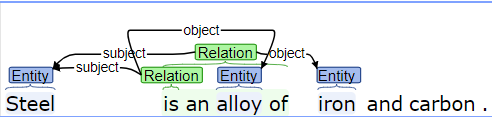
\includegraphics[width=\linewidth]{task4pas.PNG}
    \caption{Predicate-argument structure for: 'Steel is an alloy of iron and
    carbon.'}
    \label{PAStruct}
  \end{figure}
\end{enumerate}

\section{Complex Open IE, Rhetorical Strcutures}
'As the carbon percentage content rises, steel has the ability to become harder
and stronger through heat treating; however, it becomes less ductile.'
\begin{enumerate}
  \item Nucleus: 'As the carbon percentage content rises, steel has the ability
  to become harder and stronger through heat treating;'\par
  Satellite: 'however, it becomes less ductile.'
  \item Diagram: see fig. 5
  %--\begin{figure}[ht]
  %--  \includegraphics[width=\linewidth]{task5diag.PNG}
  %--  \caption{Diagram with rhetorical relations.}
  %--  \label{PAStruct}
  %--\end{figure}
  \item Hypotactic relations:
  \begin{itemize}
    \item
  \end{itemize}
  Paratactic relations:
  \begin{itemize}
    \item
  \end{itemize}
  \item RDF-NL notation of above sentence:\par
  \begin{itemize}
    \item 0 the carbon percentage content   rises
    \item 0 steel   has the ability   to become harder through heat treating
    (L:LIST)
    \item 0 steel   has the ability   to become stronger through heat treating
    (L:LIST)
  \end{itemize}
\end{enumerate}

\section{Taxonomies, Thesauri}
\begin{enumerate}
  \item WordNet glosses for martensite and austenite:
  \begin{itemize}
    \item martensite: (a solid solution of carbon in alpha-iron that is formed
    when steel is cooled so rapidly that the change from austenite to pearlite
    is suppressed; responsible for the hardness of quenched steel)
    \item austenite: (a solid solution of ferric carbide or carbon in iron;
    cools to form pearlite or martensite)
  \end{itemize}
  \item Hypernym hierarchies for martensite and austenite:\par
  They are the same from the initial definitions of both words:
  \begin{itemize}
    \item Start with either one:
    \begin{itemize}
      \item \underline{martensite}: (a solid solution of carbon in alpha-iron
      that is formed when steel is cooled so rapidly that the change from
      austenite to pearlite is suppressed; responsible for the hardness of
      quenched steel)
      \item \underline{austenite}: (a solid solution of ferric carbide or
      carbon in iron; cools to form pearlite or martensite)
    \end{itemize}
    \item \underline{solid solution}, \underline{primary solid solution}:
    (a homogeneous solid that can exist over a range of component chemicals;
    a constituent of alloys that is formed when atoms of an element are
    incorporated into the crystals of a metal)
    \item \underline{solution}: (a homogeneous mixture of two or more
    substances; frequently (but not necessarily) a liquid solution)
    "he used a solution of peroxide and water"
    \item \underline{mixture}: ((chemistry) a substance consisting of two or
    more substances mixed together (not in fixed proportions and not with
    chemical bonding))
    \item \underline{substance}: (the real physical matter of which a person
    or thing consists)
    "DNA is the substance of our genes"
    \begin{itemize}
      \item \underline{matter}: (that which has mass and occupies space)
      "physicists study both the nature of matter and the forces which govern
      it"
      \item \underline{physical entity}: (an entity that has physical
      existence)
      \item OR, instead of the above two, these three:
      \item \underline{part}, \underline{portion}, \underline{component},
      \underline{constituent}: (something determined in relation to something
      that includes it)
      "he wanted to feel a part of something bigger than himself"; "I read a
      portion of the manuscript"; "the smaller component is hard to reach";
      "the animal constituent of plankton"
      \item \underline{relation}: (an abstraction belonging to or
      characteristic of two entities or parts together)
      \item \underline{abstraction}, \underline{abstract entity}: (a general
      concept formed by extracting common features from specific examples)
    \end{itemize}
    \item \underline{entity}: (that which is perceived or known or inferred
    to have its own distinct existence)
  \end{itemize}
  \item Sibling terms for martensite: (primary solid solution, solid solution),
  austenite, ferrite, double salt\par
  Sibling terms for austenite: (primary solid solution, solid solution),
  austenite, ferrite, double salt
  \item There are 9 synsets (4 noun based, 5 verb based). The steel-related
  synsets are:
  \begin{itemize}
    \item \underline{toughness}: (the elasticity and hardness of a metal
    object; its ability to absorb considerable energy before cracking), a
    near-synonym
    \item \underline{harden}: (harden by reheating and cooling in oil)
    "temper steel", a near-synonym
    \item \underline{anneal}, \underline{normalise}: (bring to a desired
    consistency, texture, or hardness by a process of gradually heating and
    cooling) "temper glass"
  \end{itemize}
\end{enumerate}

\section{Frame Semantics - Exploring Further}
Verbs: melt, oxidise
\begin{enumerate}
  \item Frame semantics for these verbs using VerbNet, PropBank and FrameNet
  \begin{itemize}
    \item PropBank
    \begin{itemize}
      \item Roleset id, melt: to change from a solid to a liquid state, melted,
      in a (hot) liquid state
      \item Roleset id, oxidize: to (cause to) convert into an oxide, combine
      with oxygen
      \item Aliases, melt: melt, motlen
      \item Aliases, oxidize: oxidize, oxidation
      \item Roles, melt: agent, thing melted
      \item Roles, oxidize: Cause of oxidizing, Scientist causing conversion
    \end{itemize}
    \item FrameNet: both verbs return no frame results when searched for, but
    here are the differences between the lexical unit search results
    \begin{itemize}
      \item Melt:
      \begin{itemize}
        \item melt (verb), cause change of phase, finished initial
        \item melt (verb), change of phase, finished initial
        \item melt (verb), apply heat, created
        \item melt (verb), substance, finished initial
        \item melt (verb), apply heat, created
      \end{itemize}
      \item Oxidise:
      \begin{itemize}
        \item oxidise (verb), corroding caused, insufficient attestations
        \item oxidise (verb), corroding, created
      \end{itemize}
    \end{itemize}
    \item VerbNet:
  \end{itemize}
  \item Awaiting answers from Andre
  \item Awaiting answers from Andre
\end{enumerate}
\end{document}
